% Online Resource 1 Fig. S4a: the federated training loop (panel b of the former main Fig. 3, moved in the figure
% audit; panel a stays in the main paper as fig_architecture.tex). Standalone-compilable for iteration; \input{}
% into the paper body. Mirrors Papers_4-5/Paper_4/figures/fig1_architecture.tex's
% style conventions (box/arrow styles, font, palette).
\documentclass[tikz,border=2pt]{standalone}
\usepackage{amsmath}
\usetikzlibrary{arrows.meta,positioning,fit,backgrounds}

\renewcommand{\sfdefault}{phv}
\begin{document}
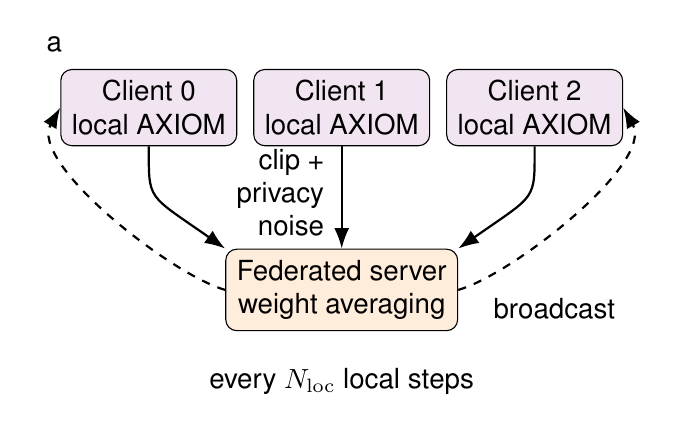
\begin{tikzpicture}[
  font=\sffamily\normalsize,
  box/.style={draw, rounded corners, minimum height=0.7cm, align=center, inner xsep=4pt, inner ysep=4pt},
  node1/.style={box, fill=blue!12, minimum width=1.0cm},
  node2/.style={box, fill=blue!12, minimum width=1.0cm},
  node3/.style={box, fill=blue!12, minimum width=1.0cm},
  encoder/.style={box, fill=orange!12, minimum width=2.6cm},
  qhead/.style={box, fill=green!12, minimum width=1.5cm, minimum height=0.55cm},
  client/.style={box, fill=violet!10, minimum width=1.8cm},
  server/.style={box, fill=orange!14, minimum width=2.0cm},
  arrow/.style={-{Latex[length=2.6mm, width=1.9mm]}, thick},
  dashedarrow/.style={-{Latex[length=2.6mm, width=1.9mm]}, thick, dashed},
]

% ===== Federated training loop =====
\node[font=\sffamily] (righttitle) at (2.6,3.0) {a};

\node[client, minimum width=1.9cm] (c1) at (3.8,2.2) {Client 0\\\normalsize local AXIOM};
\node[client, minimum width=1.9cm] (c2) at (6.25,2.2) {Client 1\\\normalsize local AXIOM};
\node[client, minimum width=1.9cm] (c3) at (8.7,2.2) {Client 2\\\normalsize local AXIOM};

\node[server, below=1.3cm of c2] (server) {Federated server\\\normalsize weight averaging};

\draw[arrow] (c1.south) .. controls +(0,-0.7) and +(-1.0,0.7) .. (server.north west);
\draw[arrow] (c2.south) -- (server.north);
\draw[arrow] (c3.south) .. controls +(0,-0.7) and +(1.0,0.7) .. (server.north east);

\draw[dashedarrow] (server.west) .. controls +(-0.7,0.2) and +(-0.4,-0.7) .. (c1.west);
\draw[dashedarrow] (server.east) .. controls +(0.7,0.2) and +(0.4,-0.7) .. (c3.east);
\node[font=\sffamily\normalsize, align=right, anchor=east] at (6.15,1.12) {clip +\\privacy\\noise};
\node[font=\sffamily\normalsize] at (8.95,-0.35) {broadcast};

\node[below=0.35cm of server, font=\sffamily\normalsize, align=center] {every $N_{\mathrm{loc}}$ local steps};

\end{tikzpicture}
\end{document}
